\section{ARDUINO VE KULLANILAN MALZEMELER}
    Bu bölümde, projede kullanılan temel bileşenler ve bu bileşenlerin çalışma prensipleri açıklanmaktadır. Projede, Arduino mikrodenetleyici kartı, L298N motor sürücü kartı, LCD ekran, DC motor, servo motor, buzzer (sesli alarm cihazı) ve HC-SR04 mesafe sensörü gibi çeşitli donanımlar kullanılmıştır.

\subsection{Arduino}

    Arduino, açık kaynaklı bir elektronik geliştirme platformudur ve temel olarak bir mikrodenetleyici kartı ile bu kartı programlamak için kullanılan yazılımdan oluşur. Şekil \ref{fig:3}'de verilen örnekte göründüğü gibi Arduino'nun en önemli avantajı, kolay öğrenilebilir olması ve geniş bir topluluk tarafından desteklenmesidir. Elektronik projelerde hızlı prototipleme ve uygulama geliştirme için yaygın bir şekilde kullanılır.
    
\begin{figure}[H]
\centering
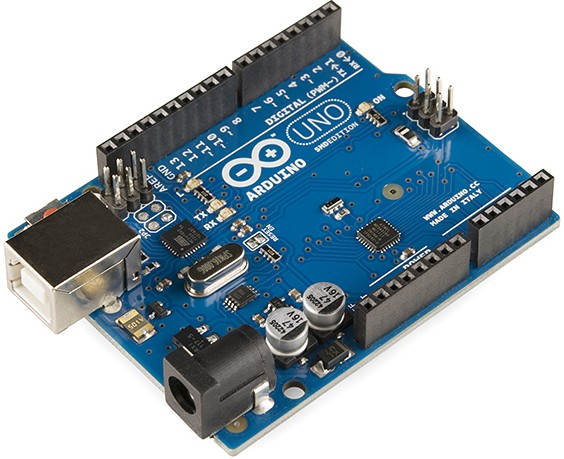
\includegraphics[width=0.50\textwidth]{Resimler/3}
\caption{Arduino Uno}
\label{fig:3}
\end{figure}
\subsubsection{Arduino'nun temel özellikleri}
    Şekil \ref{fig:6}'de verilen örnekte göründüğü gibi bütün Arduino
çeşitleri aşağıda verilen temel özelliklere sahiptir.
\begin{itemize}   
\item \textbf{Açık kaynaklı yapı:} Arduino'nun hem donanımı hem de yazılımı açık kaynaklıdır. Bu, kullanıcıların kartın tasarımını inceleyip özelleştirebilmesine olanak tanır.
\item \textbf{Kullanıcı dostu yazılım (Arduino IDE):} Arduino, kolay kullanımlı bir entegre geliştirme ortamına (IDE) sahiptir. Bu ortam, C ve C++ tabanlı bir dil kullanarak Arduino kartlarını programlamayı sağlar.
\item \textbf{Geniş modül desteği:} Sensörler, motorlar, ekranlar ve daha birçok donanımla kolayca entegre edilebilir.
\item \textbf{Düşük maliyet:} Uygun fiyatlı olması nedeniyle hem amatörler hem de profesyoneller tarafından tercih edilir.
\item \textbf{Kapsamlı Topluluk Desteği:} Çevrimiçi topluluklarda geniş bir destek ağı bulunur. Arduino projeleri için birçok hazır kütüphane ve örnek bulunmaktadır.
\end{itemize}

    
\begin{figure}[H]
\centering
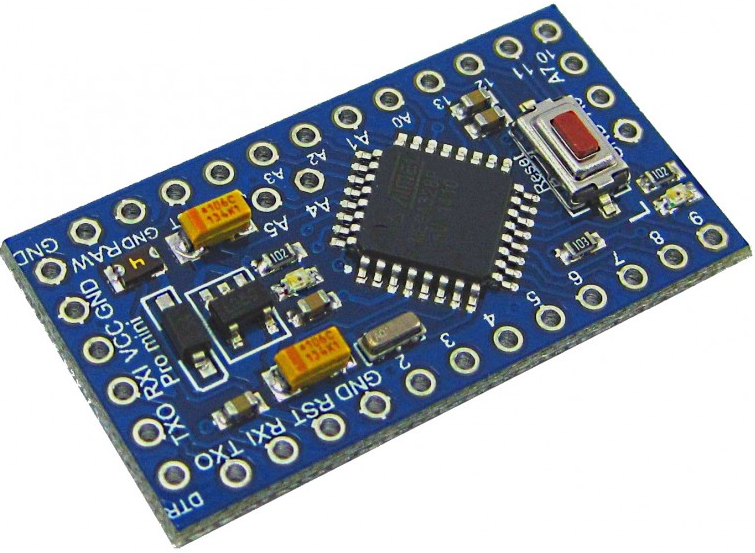
\includegraphics[width=0.45\textwidth]{Resimler/6.png}
\caption{Arduino Pro Mini 328}
\label{fig:6}
\end{figure}
\subsubsection{Arduino'nun çalışma prensibi}
   
    Arduino, fiziksel dünya ile dijital dünya arasında bir köprü görevi görür. Kart üzerindeki giriş ve çıkış pinleri sayesinde sensörlerden veri alabilir ve motorlar, LED'ler gibi cihazları kontrol edebilir. Arduino'nun temel işleyişi şu şekildedir:
\begin{itemize}
\item Sensörlerden gelen analog veya dijital sinyaller alınır.
\item Bu sinyaller, mikrodenetleyici (ör. ATmega328P) tarafından işlenir.
\item İşlenen verilere göre çıkış cihazlarına (motor, ekran, buzzer vb.) komutlar gönderilir.
\end{itemize}

\subsubsection{Arduino çeşitleri}
    Arduino platformunda birçok farklı model bulunmaktadır. Her model, farklı ihtiyaçlara yönelik olarak tasarlanmıştır;
\begin{itemize}   

\item \textbf{Arduino uno:} Arduino şekil \ref{fig:7}'de verilen örnekte göründüğü gibi platformunun en popüler ve en çok kullanılan modelidir. Eğitim ve prototip geliştirme için uygundur.
\par\textbf{\textit{\underline{Arduino uno teknik özellikleri:}}}

\begin{itemize}
\item \textbf{Mikrodenetleyici:} ATmega328P
\item \textbf{Çalışma gerilimi:} 5V
\item \textbf{Giriş voltajı:} 7-12V
\item \textbf{Dijital I/O pin sayısı:} 14 (6 tanesi PWM çıkış destekler)
\item \textbf{Analog giriş sayısı:} 6
\item \textbf{Flash hafıza:} 32 KB (0.5 KB'si bootloader için ayrılmıştır)
\item \textbf{SRAM:} 2 KB
\item \textbf{EEPROM:} 1 KB
\item \textbf{Saat hızı:} 16 MHz
\end{itemize}


\begin{figure}[H]
\centering
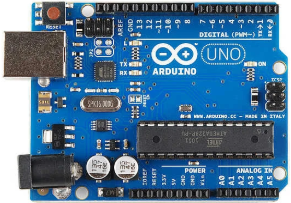
\includegraphics[width=0.45\textwidth]{Resimler/7.png}
\caption{Arduino Uno}
\label{fig:7}
\end{figure}

\item \textbf{Arduino mega:} Arduino Mega, şekil \ref{fig:8}'de verilen örnekte göründüğü gibi daha fazla giriş/çıkış pinine ve daha geniş hafızaya ihtiyaç duyulan projeler için geliştirilmiştir.
\begin{figure}[H]
\centering
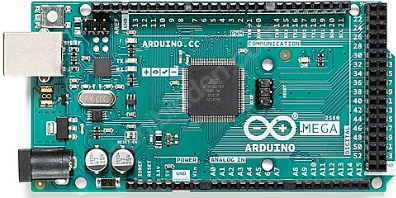
\includegraphics[width=0.50\textwidth]{Resimler/8.png}
\caption{Arduino Mega}
\label{fig:8}
\end{figure}
{}
\item \textbf{Arduino nano:} Arduino Nano, şekil \ref{fig:9}'de verilen örnekte göründüğü gibi küçük projeler için tasarlanmış kompakt bir modeldir.
\begin{figure}[H]
\centering
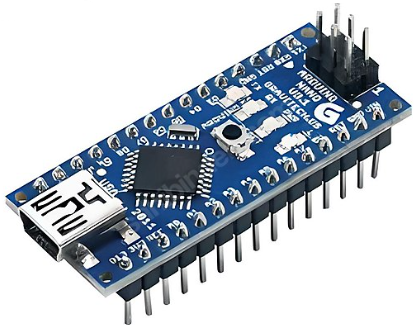
\includegraphics[width=0.50\textwidth]{Resimler/9.png}
\caption{Arduino Nano}
\label{fig:9}
\end{figure}

\item \textbf{Arduino MKR serisi:} Arduino MKR serisi, şekil \ref{fig:10}'de verilen örnekte göründüğü gibi 32-bit ARM tabanlı bir mikrodenetleyiciye sahiptir ve yüksek işlem gücü gerektiren projeler için uygundur.
\begin{figure}[H]
\centering
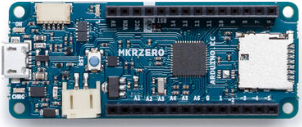
\includegraphics[width=0.50\textwidth]{Resimler/10}
\caption{Arduino MKR Serisi}
\label{fig:10}
\end{figure}

\end{itemize}

\subsection{L298N Motor Sürücü Kartı}
    L298N, çift kanallı bir motor sürücü entegresi olup, özellikle DC motorlar ve step motorlar gibi motorları kontrol etmek için tasarlanmış bir modüldür. H-köprüsü (H-Bridge) prensibiyle çalışan bu entegre, motorların hem yönünü (ileri/geri) hem de hızını (PWM ile) kontrol etme imkânı sağlar. Şekil \ref{fig:12}'de verilen örnekte göründüğü gibi L298N motor sürücü kartı, bu entegrenin kullanımını kolaylaştıran bir modül olarak sunulur.

\begin{figure}[H]
\centering
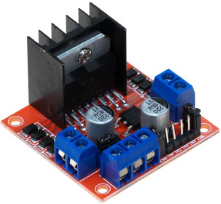
\includegraphics[width=0.45\textwidth]{Resimler/12.png}
\caption{L298N Motor Sürücü Kartı}
\label{fig:12}
\end{figure}

\subsubsection{L298N motor sürücü kartının özellikleri}
\begin{itemize}   
\item \textbf{Çift Kanallı Çıkış:} L298N, aynı anda iki motoru kontrol edebilir. Her motor için bağımsız yön ve hız kontrolü yapılabilir.
\item \textbf{H-Köprüsü Yapısı:} H-köprüsü, bir motorun her iki yönde de dönmesini sağlayan bir devre yapısıdır. L298N, bu yapıyı içeren bir entegre olduğu için motor yön kontrolü kolayca yapılabilir.
\item \textbf{Yüksek Akım Kapasitesi:} Her kanal başına maksimum 2A sürekli akım sağlayabilir ve kısa süreli tepe akımı daha yüksektir.
\item \textbf{Geniş Çalışma Gerilimi:} 5V ile 35V arasında çalışabilir, bu da hem düşük gerilimli hem de yüksek gerilimli motorlar için uygun olmasını sağlar.
\item \textbf{Entegre Soğutucu:} Yüksek akımlarda ısınmayı önlemek için genellikle bir soğutucu ile gelir.
\end{itemize}

\subsubsection{L298N motor sürücü kartının teknik özellikleri}

\begin{itemize}
\item \textbf{Çalışma gerilimi:} 5V - 35V
\item \textbf{Maksimum akım:} 2A (kanal başına)
\item \textbf{Kontrol tipi:} Dijital sinyaller (PWM)
\item \textbf{Motor türleri:}
\begin{itemize}
\item DC Motor (Hız ve yön kontrolü)
\item Step Motor (Adım ve yön kontrolü)
\end{itemize}
\end{itemize}

\subsubsection{L298N motor sürücü kartının avantajları ve dezavantajları}
\textbf{\textit{\underline{Avantajları:}}}
\begin{itemize}
\item Çift motor kontrolü sayesinde ekonomik ve çok yönlüdür.
\item Hem DC hem de step motorlarla çalışabilir.
\item PWM ile hız kontrolü yapabilir.
\end{itemize}

\textbf{\textit{\underline{Dezavantajları:}}}
\begin{itemize}
\item Yüksek akım çeken motorlarda aşırı ısınma meydana gelebilir.
\item Güncel motor sürücülere göre enerji kaybı daha fazladır (verimlilik açısından).
\item Düşük hızlı çalışmalarda motor titreşimi artabilir.
\end{itemize}

\subsubsection{L298N motor sürücü kartının pinlerin açıklamaları}
\begin{itemize}
\item \textbf{ VCC:} Motorun güç kaynağına bağlanır (5V-35V).
\item \textbf{GND:}  Ortak toprak bağlantısıdır.
\item \textbf{5V:} Modülün lojik devresini beslemek için kullanılır (opsiyonel).
\item \textbf{IN1 ve IN2:} Motor 1'in yön kontrol pinleri:
\begin{itemize}
\item IN1 yüksek, IN2 düşük ise motor ileri döner.
\item IN1 düşük, IN2 yüksek ise motor geri döner.
\end{itemize}
\item \textbf{IN3 ve IN4:} Motor 2'nin yön kontrol pinleri (benzer şekilde çalışır).
\item \textbf{EN1:} Motor 1'in hız kontrolü için PWM sinyali bağlanır.
\item \textbf{EN2:} Motor 2'nin hız kontrolü için PWM sinyali bağlanır.

\end{itemize}
\subsection{LCD}
    LCD, sıvı kristal maddelerin ışık geçirme özelliklerini kullanan bir ekran teknolojisidir. Sıvı kristaller, elektriksel bir gerilim uygulandığında ışık geçişini değiştirebilen maddelerdir. Bu özellik, LCD ekranların görüntü oluşturmasını sağlar. Şekil \ref{fig:14}'de verilen örnekte göründüğü gibi LCD ekranlar, arka aydınlatma (genellikle LED) ve sıvı kristal katmanlardan oluşur. LCD ekranlarda, sıvı kristaller ışığı yönlendirebilir veya engelleyebilir, bu sayede görüntü oluşur.

\begin{figure}[H]
\centering
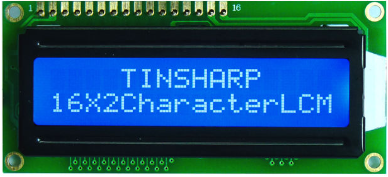
\includegraphics[width=0.65\textwidth]{Resimler/14.png}
\caption{Lcd}
\label{fig:14}
\end{figure}

\subsubsection{LCD özellikleri}
\begin{itemize}   
\item \textbf{Yüksek görüntü kalitesi:} LCD ekranlar, yüksek çözünürlük ve netlik sunar. Piksel yoğunluğu arttıkça, ekran daha keskin ve ayrıntılı görüntüler gösterir. Renk doğruluğu oldukça iyidir, ancak kontrast oranı CRT ekranlara kıyasla daha düşüktür.
\item \textbf{Düşük güç tüketimi:} LCD ekranlar, diğer ekran teknolojilerine (örneğin CRT) göre çok daha düşük enerji tüketir. Bu, özellikle taşınabilir cihazlarda batarya ömrünü uzatır.
\item \textbf{Yüksek kontrast oranı:} LCD ekranlar, siyah ve beyaz arasındaki farkları belirgin şekilde ayırabilir. Ancak, bu özellik OLED veya AMOLED ekranlarla karşılaştırıldığında biraz daha sınırlıdır.
\item \textbf{Renk derinliği:} LCD ekranlar genellikle 16.7 milyon renk (24-bit renk derinliği) sunar. Bu, zengin ve doğru renklerin ekran üzerinde görüntülenmesini sağlar.
\end{itemize}

\subsubsection{LCD I2C modülü}
I2C modülü, I2C protokolü kullanarak veri iletimi sağlayan bir arayüzdür. LCD ekranın veri iletimi için I2C modülü kullanıldığında, ekranın 4 pin yerine 4 veya 5 pin ile kontrol edilmesi mümkün olur. Şekil \ref{fig:15}'de verilen örnekte göründüğü gibi, kablo karmaşasını azaltır ve bağlantıları daha basit hale getirir.
\par\textbf{\underline{I2C modülünün pinleri}}
\begin{itemize}
\item \textbf{VCC:} Güç (5V)
\item \textbf{GND:} Toprak (Ground)
\item \textbf{SDA:} Veri hattı (Serial Data Line) (A4)
\item \textbf{SCL:} Saat hattı (Serial Clock Line) (A5)
\item \textbf{V0:} Kontrast ayarı (Opsiyonel, bazı modellerde bulunabilir)
\end{itemize}

\begin{figure}[H]
\centering
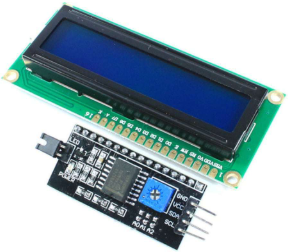
\includegraphics[width=0.50\textwidth]{Resimler/15.png}
\caption{LCD with I2C}
\label{fig:15}
\end{figure}

\subsection{Ultrasonik Mesafe Sensörü}
    Ultrasonik mesafe sensörü, ses dalgalarını kullanarak bir nesne ile sensör arasındaki mesafeyi ölçen bir cihazdır. Şekil \ref{fig:17}'de verilen örnekteki sensörler, genellikle HC-SR04 gibi modüllerle kullanılır ve ultrasonik dalgalar (yani insan kulağının duyamayacağı frekansta ses dalgaları) gönderip geri dönen dalgaların süresini ölçerek mesafeyi hesaplar. Bu sensörler çok yaygın olarak robotik uygulamalar, mesafe ölçümü ve engel algılama sistemlerinde kullanılır.

\begin{figure}[H]
\centering
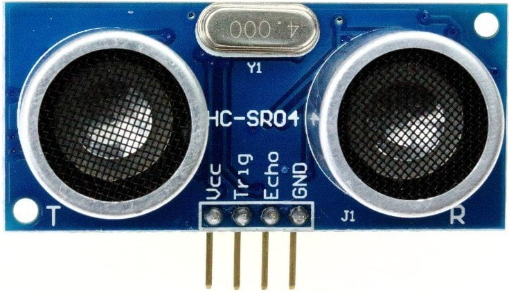
\includegraphics[width=0.45\textwidth]{Resimler/17.png}
\caption{HC-SR04 Ultrasonik Mesafe Sensörü}
\label{fig:17}
\end{figure}

\subsubsection{Ultrasonik mesafe sensörü çalışma prensibi}

\begin{itemize}
\item \textbf{Trig (Tetikleme) pinine sinyal gönderme:} Sensör, belirli bir süre boyunca trig pinine yüksek sinyal gönderir. Bu sinyal, ultrasonik dalganın yayılmasını başlatır.
\item \textbf{Ultrasonik dalgaların yansıması:} Ultrasonik dalgalar bir nesneye çarptığında geri yansır.
\item \textbf{Echo (Yankı) pininden geri dönüş süresi ölçülmesi:} Geri dönen yankının zamanını ölçen echo pini, bu süreyi Arduino'ya bildirir.
\item \textbf{Mesafe hesaplama:} Yansıyan dalgaların geri dönüş süresi, ses dalgasının hızına (yaklaşık olarak 343 m/s) göre mesafeyi hesaplamak için kullanılır. Hesaplama şu formülle yapılır:

\par\underline{Mesafe= ( Süre * Ses Hızı ) / 2}
\centering
\par Burada, süre * ses hızı, ses dalgasının gidiş-dönüş yolculuğunun toplam süresi olduğu için ikiye bölünür.
\end{itemize}

\subsection{Servo Motor}

    Servo motor, şekil \ref{fig:20}'de verilen örnekte göründüğü gibi pozisyon, hız veya tork gibi parametrelerin hassas bir şekilde kontrol edilmesine olanak tanıyan bir motor türüdür. İçerisinde genellikle bir motor, bir geri bildirim sensörü (örneğin, potansiyometre veya enkoder), bir kontrol devresi ve bir sürücü bulunur.
\begin{figure}[H]
\centering
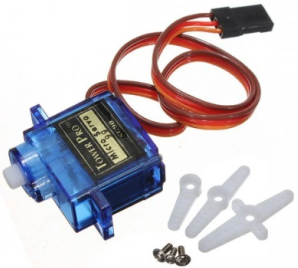
\includegraphics[width=0.45\textwidth]{Resimler/20.png}
\caption{SG90 Mini Servo Motor}
\label{fig:20}
\end{figure}

\subsubsection{Servo motorun çalışma prensibi}
    Servo motorlar, bir hedef pozisyona ulaşmak için geri besleme kontrolü kullanır. Kontrol devresi, motorun mevcut konumunu hedef konumla karşılaştırarak gerekli düzeltmeleri yapar. Temel olarak şu aşamalardan oluşur:
\begin{itemize}   
\item \textbf{Hedef sinyali:} Bir kontrol cihazından gelen komut sinyali.
\item \textbf{Geri besleme:} Motorun mevcut pozisyonunu ölçen sensör verisi.
\item \textbf{Hata sinyali:} Hedef ve mevcut pozisyon arasındaki fark.
\item \textbf{Düzeltme:} Motorun hareketini kontrol ederek hedefe ulaşır.
\end{itemize}

\subsubsection{Servo motorun avantajları ve dezavantajları}
\textbf{\textit{\underline{Avantajları}}}
\begin{itemize}   
\item Yüksek hassasiyet ve doğruluk.
\item Küçük boyutlarda güçlü performans.
\item Çeşitli kontrol seçenekleri.
\end{itemize}
\par\textbf{\textit{\underline{Dezavantajları}}}
\begin{itemize}   
\item Daha karmaşık kontrol devreleri gerektirir.
\item Göreceli olarak maliyetli.
\item Aşırı yük altında performans kaybı yaşanabilir.
\end{itemize}

\subsection{Dc Motor}

    DC (Doğru Akım) motorlar, şekil \ref{fig:22}'de verilen örnekte göründüğü gibi, doğru akımın elektrik enerjisini mekanik enerjiye dönüştüren cihazlardır. Basit yapıları, kolay kontrol edilebilirlikleri ve geniş uygulama alanları nedeniyle endüstriyel ve günlük hayatta sıkça tercih edilir.
\begin{figure}[H]
\centering
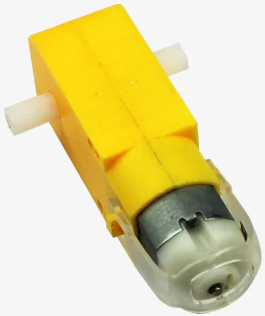
\includegraphics[width=0.35\textwidth]{Resimler/22.png}
\caption{DC Motor}
\label{fig:22}
\end{figure}

\subsubsection{DC motorun çalışma prensibi}
    DC motorun çalışma prensibi, elektrik akımının bir manyetik alan içinde hareket eden iletkenler üzerinde bir kuvvet oluşturmasıdır. Bu kuvvet, motorun rotorunu döndürerek mekanik hareket sağlar. Temel bileşenleri:
\begin{itemize}   
\item \textbf{Stator:} Sabit manyetik alan oluşturan kısım
\item \textbf{Rotor (Armatür):} Dönen kısım.
\item \textbf{Komütatör:} Akımın yönünü değiştirerek sürekli dönme sağlar.
\item \textbf{Fırçalar:} Komütatöre enerji aktaran parçalar.
\end{itemize}

\subsubsection{DC motorun avantajları ve dezavantajları}
\par\textbf{\textit{\underline{Avantajları}}}
\begin{itemize}   
\item Hızlı tepki süresi.
\item Geniş hız aralığında çalışabilir.
\item Basit ve sağlam yapı.
\end{itemize}
\par\textbf{\textit{\underline{Dezavantajları}}}
\begin{itemize}   
\item Fırçalı motorlar için bakım gereklidir.
\item Aşırı yükte performans kaybı yaşanabilir.
\item Fırçalı motorlarda gürültü ve kıvılcım oluşabilir.
\end{itemize}

\subsection{Buzzer}

    Buzzer, elektrik sinyalini ses sinyaline dönüştüren bir elektronik bileşendir. Uyarı sistemlerinde, sesli geri bildirim sağlayan devrelerde ve çeşitli elektronik cihazlarda yaygın olarak kullanılır. İki ana türü vardır: \textbf{aktif buzzer} (şekil \ref{fig:23}'de verilen örnekte göründüğü gibi) ve \textbf{pasif buzzer}.
\begin{figure}[H]
\centering
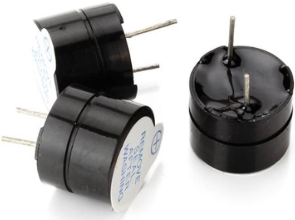
\includegraphics[width=0.45\textwidth]{Resimler/23.png}
\caption{Buzzer}
\label{fig:23}
\end{figure}

\subsubsection{Buzzer türleri}
\par\textbf{\textit{Aktif buzzer}}
\begin{itemize}   
\item Harici bir sürücü devresine ihtiyaç duymadan çalışır..
\item Sadece bir doğru akım (DC) kaynağı ile çalıştırılabilir.
\item Kullanımı kolaydır ve genellikle sabit bir frekansta ses çıkarır.
\end{itemize}
\par\textbf{\textit{Pasif buzzer}}
\begin{itemize}   
\item Harici bir sürücü sinyaline ihtiyaç duyar.
\item Ses frekansı, verilen sinyale bağlı olarak değişir.
\item Daha esnek ses kontrolü sağlar.
\end{itemize}

\subsubsection{Buzzer çalışma prensibi}
    Buzzer, piezoelektrik malzeme veya elektromanyetik prensiplerle çalışır:
\par\textbf{Piezoelektrik buzzer:}
\begin{itemize}   
\item Piezoelektrik malzeme, elektrik sinyali uygulandığında titreşir ve bu titreşim ses dalgaları oluşturur.
\item Hafif ve enerji verimlidir.
\end{itemize}
\textbf{Elektromanyetik buzzer:}
\begin{itemize}   
\item Bir bobin içindeki elektromanyetik alan, bir diyaframın titreşmesini sağlar ve bu titreşim ses üretir.
\item Genellikle daha yüksek ses seviyelerine sahiptir.
\end{itemize}